\subsection{Frontend}\label{sec:frontend}

We developed an Android application to utilize our \gls{api} as outlined in the introduction. The app serves as a reference implementation for connecting the backend functions shown in \autoref{sec:backend}.

The following requirements were defined by us in advance:

\begin{itemize}
    \item Filter for geographic location and a radius, minimal frequency of measurements (\gls{qos} aspects)
    \item Quick overview of the sensors in a smart city (around location)
    \item Capability to display sensors metadata and the measured values
\end{itemize}

\begin{figure}[H]
    \centering
    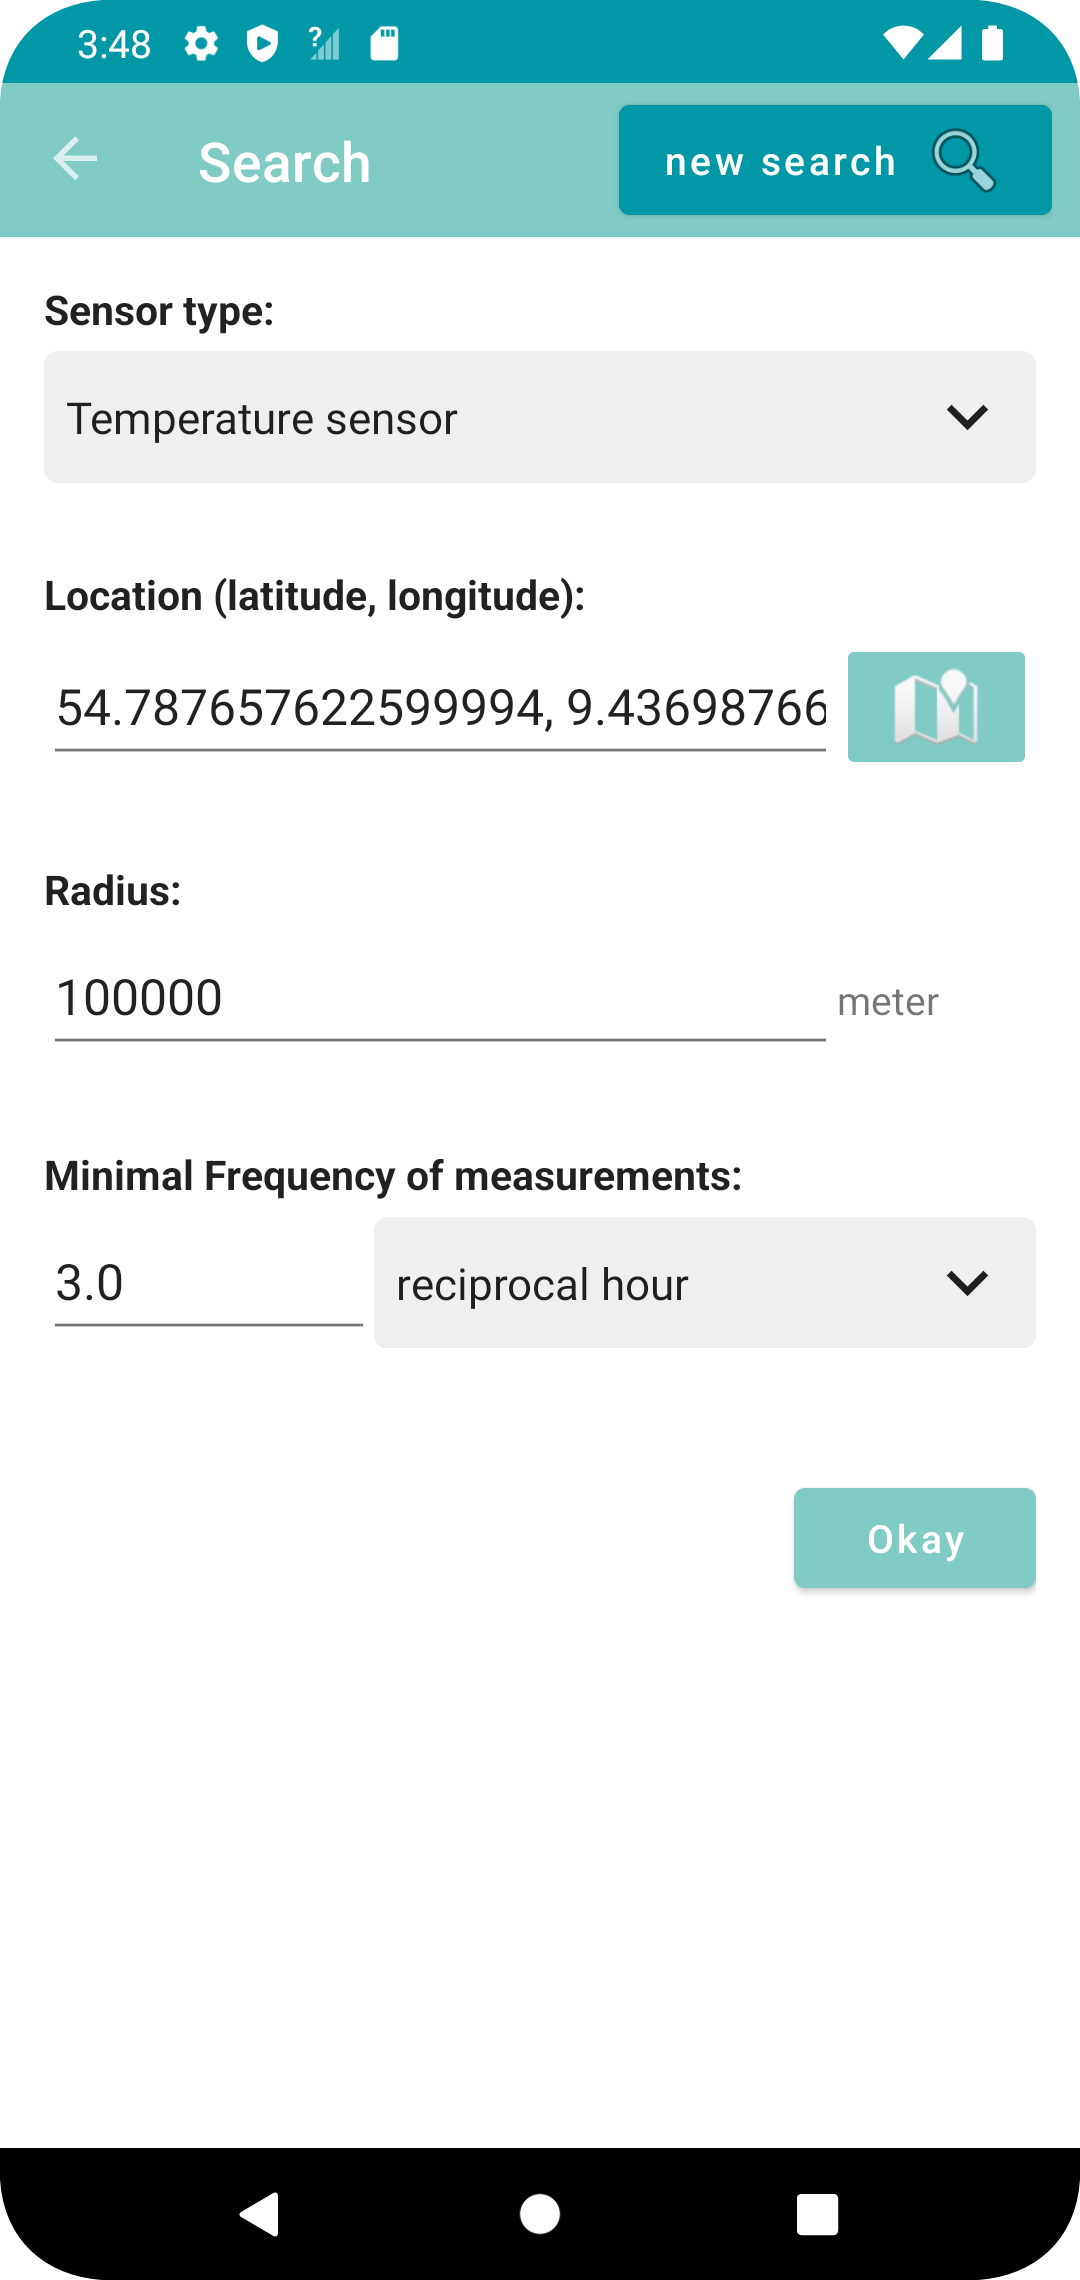
\includegraphics[scale=0.1]{screen_filter}
    \caption{Filter view}
    \label{fig:screen_main}
    \Description{
        The filter view offers the option to filter by sensor type, radius around a location, and minimum frequency of measured values. The location can be specified in longitude and latitude, or selected from a map. The unit for the frequency can be selected from a dropdown menu; the unit for the radius is meters.
    }
\end{figure}

In order to meet the requirements, we developed a filter view, which is shown in \autoref{fig:screen_main}. The view offers the option to filter by sensor type, radius around a location, and minimum frequency of measured values. The location can be specified in longitude and latitude, or selected from a map.

\begin{figure}[H]
    \centering
    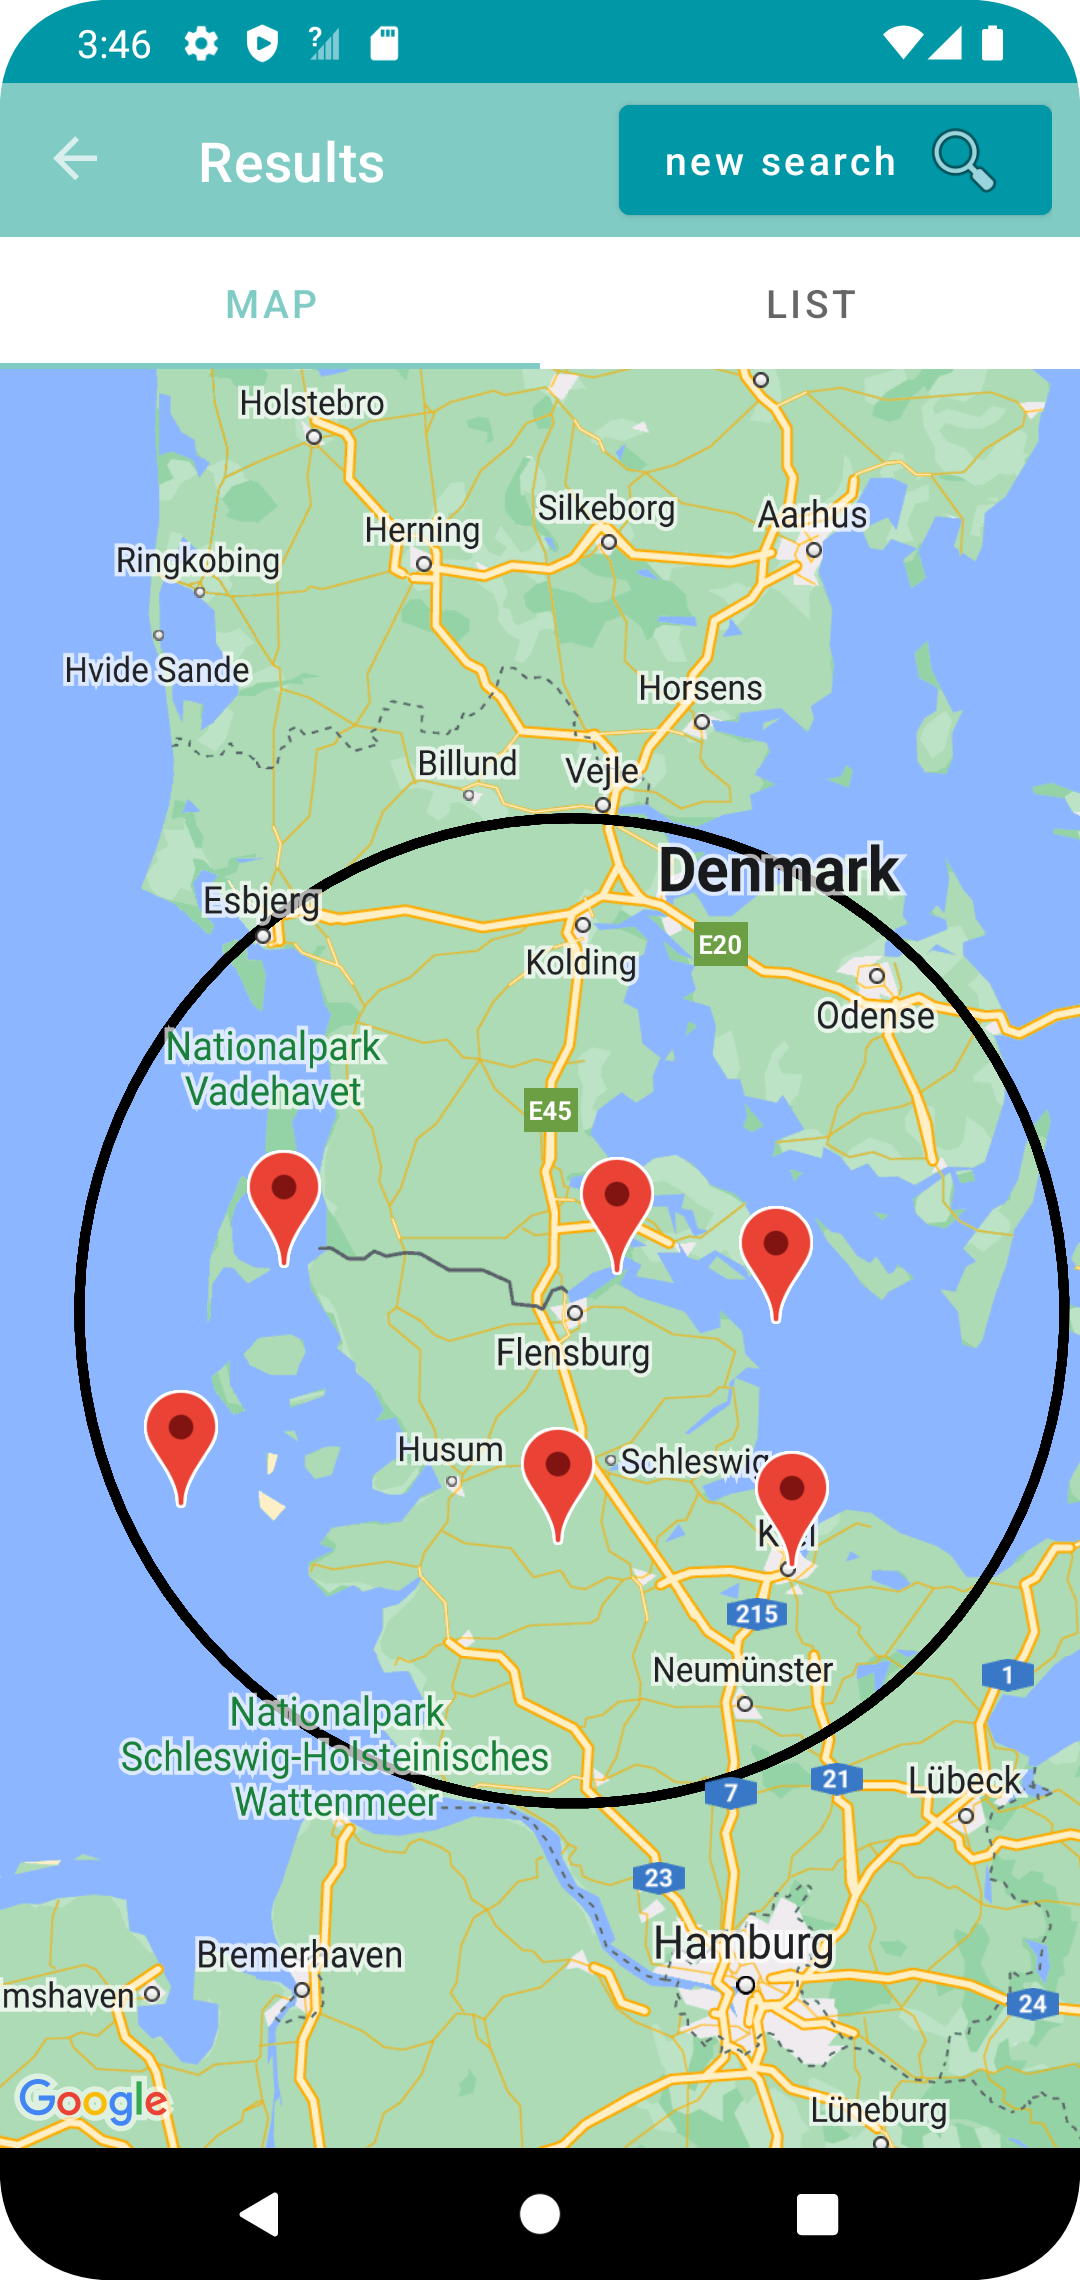
\includegraphics[scale=0.1]{screen_map}
    \caption{Map view showing the results}
    \label{fig:screen_results_map}
    \Description{
        The map view shows the sensors that match the filter criteria as well as a circle that represents the search area.
    }
\end{figure}

The sensors can be presented in a map or list view. This gives the user a quick overview of the surrounding sensors.

\begin{figure}[H]
    \centering
    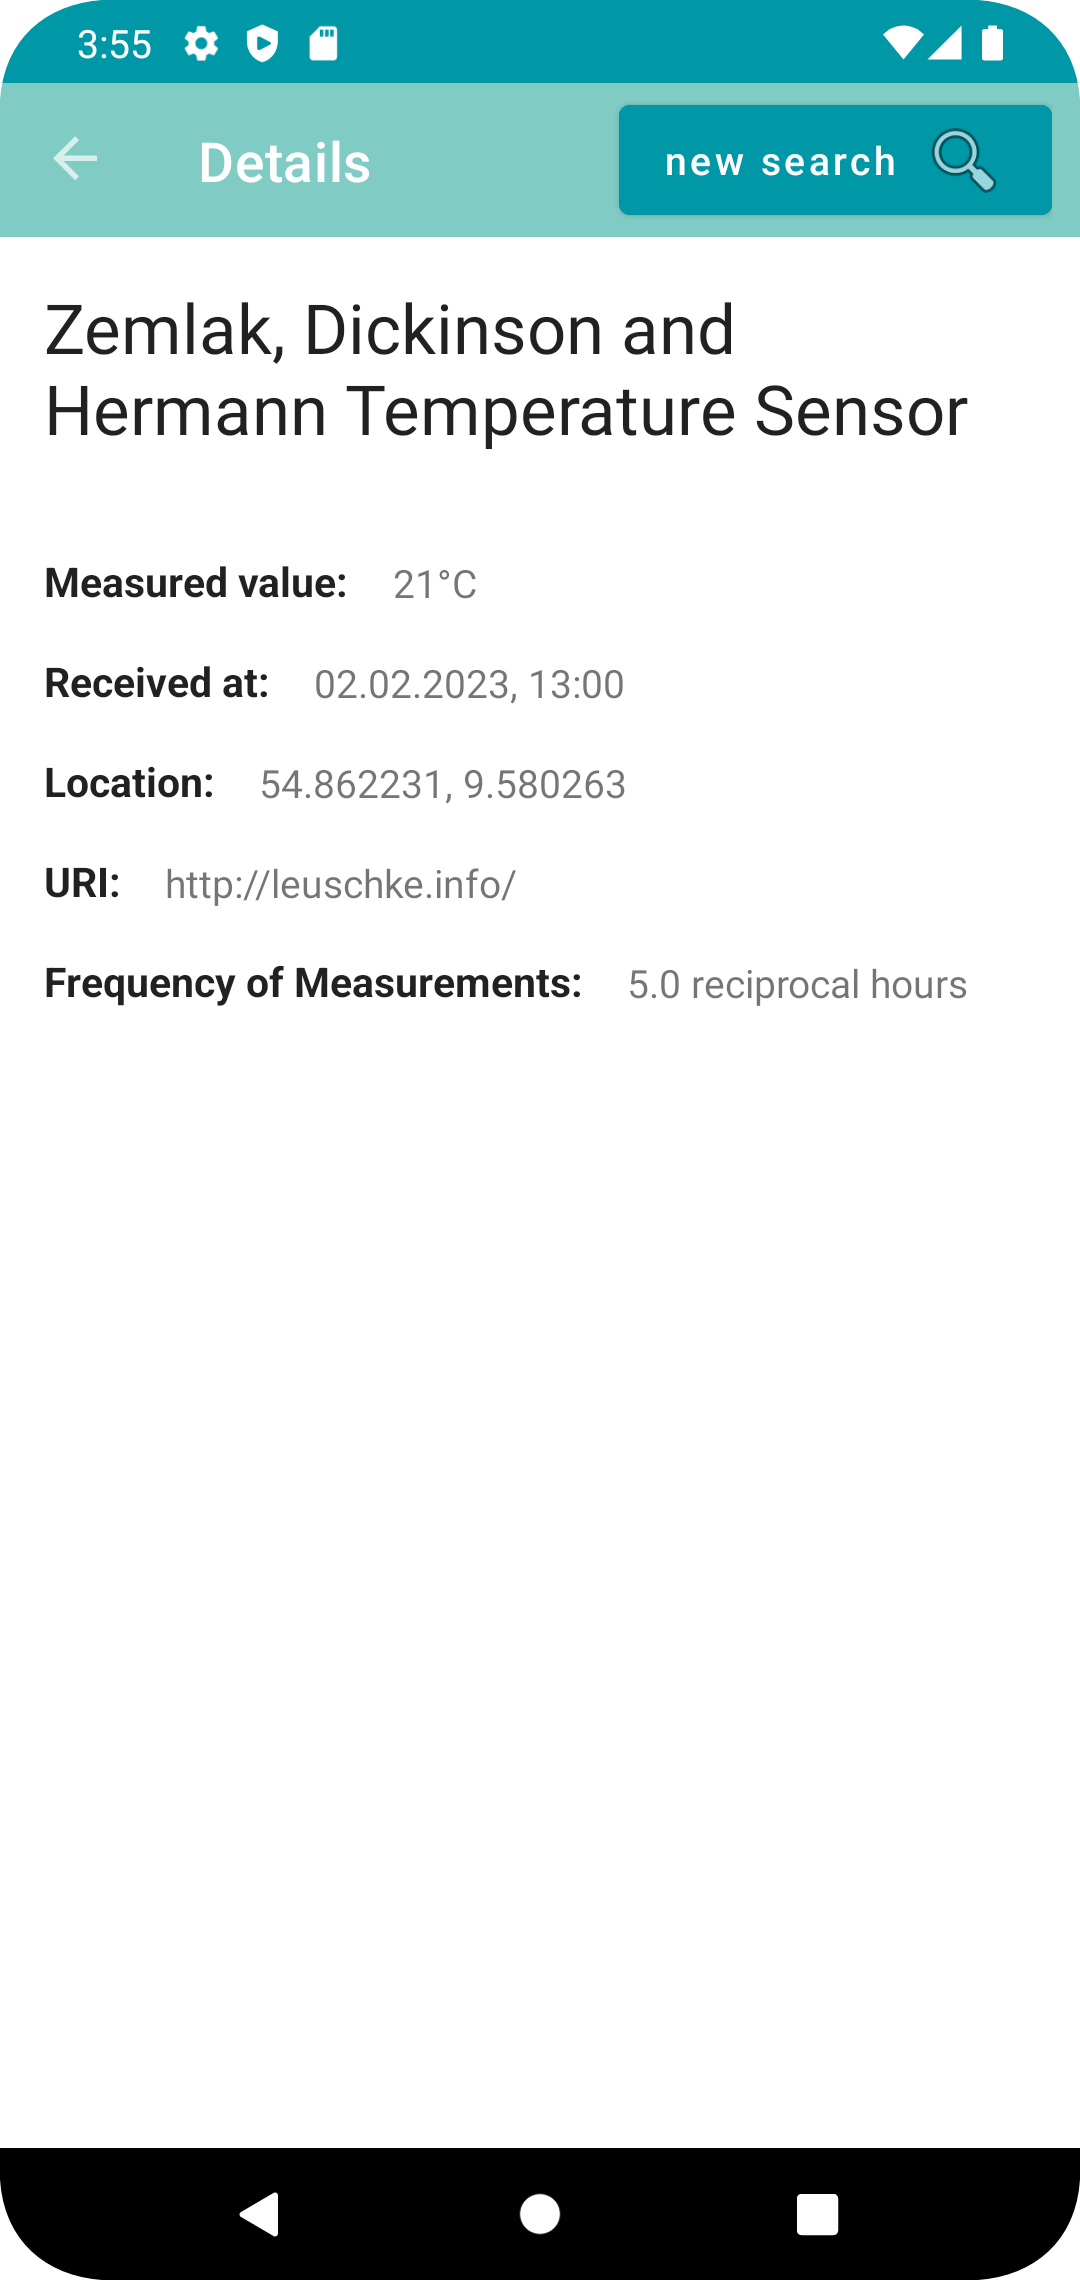
\includegraphics[scale=0.1]{screen_detail}
    \caption{Detail view of a sensor}
    \label{fig:screen_result_details}
    \Description{
        The detail view shows the metadata of the sensor and the most recent measured value.
    }
\end{figure}

The measured values and metadata will be displayed in a detailed view. It reads the data from the \gls{td} and presents them clearly to the user.

\subsubsection{JSON-LD}\label{sec:jsonld}

Since the server may hold heterogeneous data from different providers, the structure of \gls{jsonld} documents may vary, which prevents direct decoding. It first has to be normalized by expanding the data. Normalization with a different method, which could result in simpler data structures, may not work, because it could result in heterogeneous data. For example, multiple values for the same property would be encoded as an array, while a single value would be encoded as-is. Expansion would always result in an array of values, even if only a single value is present.


% TODO: App als Quelle verfügbar machen (für Veröffentlichung)
